%----------------------------------------------------------------------------
\chapter{Graph Engine}
%----------------------------------------------------------------------------

A Graph Engine a Microsoft cég egyik projektje, ami 2010. október 30. óta érhető el, akkor még \emph{Trinity} néven.\cite{MicrosoftTrinity} Ez egy gráfadatbázis-rendszer ami memóriafelhőn fut. A memóriafelhő egy globálisan címezhető, memóriában található kulcs-érték tároló. Mivel memóriaalapú, ezért gyors véletlen elérést biztosít nagyméretű gráfok esetén is, támogatja a gyors gráfbejárást és a párhuzamos feldolgozást is.\cite{Trinity}

Az elkészített megoldás Microsoft Windows 7 x64 operációs rendszeren, Visual Studioban készült és \Csh{} nyelven, ezért a továbbiakban leírtak erre a környezetre vonatkoznak.


\section{A Graph Engine felépítése}

A Graph Engine a számítógépek feladatkörét tekintve három részből áll. Vannak \emph{client}-ek, \emph{proxy}-k és \emph{slave}-k. A \emph{slave}-k hálózatba kötött szerver számítógépek, amik az adattárolásért és a lekérdezések feldolgozásáért felelősek, egymással egy hálózaton kommunikálnak. A \emph{client}-ek felelőssége egy felhasználói felületet adni az adatbázishoz. A \emph{proxy}-k az üzenetek kezelését végzik, de nem feltétlenül szükségesek a kommunikációhoz, a \emph{client}-ek is képesek közvetlenül a szerverrel kommunikálni. A Graph Engine lehetőséget kínál mindezen szerepek egy számítógépen való futtatásához is.


\section{TSL}

A \emph{TSL}, azaz \emph{Trinity Specification Language} a Graph Engine gráfséma-leíró nyelve. Az előre definiált adatstruktúra helyett nagy könnyebbséget kínál azáltal, hogy szerveroldalon az adott alkalmazásra specifikus adatstruktúrát adhatunk meg. Szintaxisát tekintve leginkább a C, \cpp{}  és a \Csh{} nyelvre hasonlít.

A \emph{TSL} lehetőséget kínál sokfajta beépített típus használatára, melyek a következők:
\begin{itemize}
	\item \texttt{bool} \--- logikai
	\item \texttt{char} \--- karakter
	\item \texttt{int8, uint8, int16, uint16, int32, uint32, int64, uint64} \--- egész szám 
		
		Az \texttt{u} azt jelöli, hogy előjel nélküli, a szám pedig azt, hogy hány bites.
	\item \texttt{CellId} \--- 64 bites előjeles egész szám
		
		A különbség a \texttt{Cellid} és az \texttt{int64} között a programozó irányába hordozott jelentésben van. A \texttt{CellId}-t cellák egyedi azonosítójára való hivatkozásra használják.
	\item \texttt{float, double} \--- lebegőpontos szám
		A \texttt{float} 32, a \texttt{double} 64 bites.
	\item \texttt{decimal} \--- fix pontosságú szám 128 biten tárolva
	\item \texttt{DateTime} \--- dátum
	\item \texttt{Guid} \--- 128 bites egyedi azonosító
\end{itemize}

A Graph Engine egy ilyen \emph{TSL} fájl alapján építi fel az adatbázis sémáját. Ennek a fájlnak a kiterjesztése \emph{.tsl} és a következő elemekből épül fel:
\begin{itemize}
	\item \texttt{include \ldots{}} \--- Az \emph{include} után megadott fájlt ennek a fájlnak az elejére fűzi.
	\item \texttt{enum\{\ldots{} \}} \--- Felsorolás típust írhatunk le benne hasonlóan, mint C-ben.
	\item \texttt{struct structNeve \{\ldots{} \}} \--- Személyre szabható típus. Beépített típusok, konténerek és más \texttt{struct}-ok helyezhetőek el benne. A \emph{TSL} háromféle konténer típust támogat:
	\begin{itemize}
		\item \texttt{Array<T>} \--- T típusú elemek tömbje. Csak beépített típust támogat.
		\item \texttt{List<T>} \--- T típusú elemek listája. Előnye a tömbbel szemben, hogy dinamikus méretű elemek (konténerek) is tárolhatóak benne. A \Csh{}-ban lévő \texttt{List<T>}-nek megfeleltethető.
		 \item \texttt{string} \--- Karakterek sorozatát lehet benne tárolni.
	\end{itemize}
	\item \texttt{cell cellaNeve\{\ldots{} \}} \--- Struktúráját tekintve hasonló a \texttt{struct} típushoz, ellenben minden \texttt{cell}-hez tartozik egy egyedi azonosító (\texttt{CellId}), amin keresztül hivatkozni lehet rá. 
	\item Attribútumok \--- Stringek kulcs-érték párosa. Segítségükkel futási idejű információt lehet adni az adott celláról vagy mezőjéről.
	\item \texttt{protocol, server, proxy} \--- Távoli adatbázis-elérést lehet velük konfigurálni.
\end{itemize}

A \emph{TSL}-t külön projektbe kell elhelyezni. Fordítása után egy \emph{dll} könyvtár jön létre, amit a másik \Csh{} projektünkhöz hozzálinkelhetünk. Amennyiben a Graph Engine beépített projektjét használjuk és egy \emph{solution} alatt dolgozunk, akkor ezt a Visual Studio elvégzi helyettünk.

Lehetőség van úgynevezett \emph{Attribute}-okat hozzáadnunk a \emph{TSL} fájlhoz. Ezek \emph{string} típusú kulcs-érték párok, melyek a programozó számára információval látják el az egyes tulajdonságokat. Érdemes ilyen módon megjelölni a gráf éleit. Ez csak egy futásidőben elérhető információval látja el a csúcsokat. Szintaxisa \texttt{[kulcs:érték]} alakú. A kettőspont és az érték elhagyható.

\subsection{Példa TSL fájlra}

A példában egy baráti társaságban lévő emberekről tárolunk adatokat. Ezek az adatok legyenek a következők minden embernél: név, személyiigazolvány-szám, barátok. Sokféle megoldás létezhet ennek a problémának a leírására, mivel a nevet tárolhatjuk egy \texttt{string}-ben, de akár egy struktúrában is, a személyiigazolvány-szám lehet fix hosszúságú 6 karakter vagy lehet egy változó hosszú \texttt{string}. Esetünkben a név egy struktúra, titulussal, vezetéknévvel és keresztnévvel, a  személyiigazolvány-szám pedig \texttt{string} típusú.

\begin{figure}[H]
	\centering
	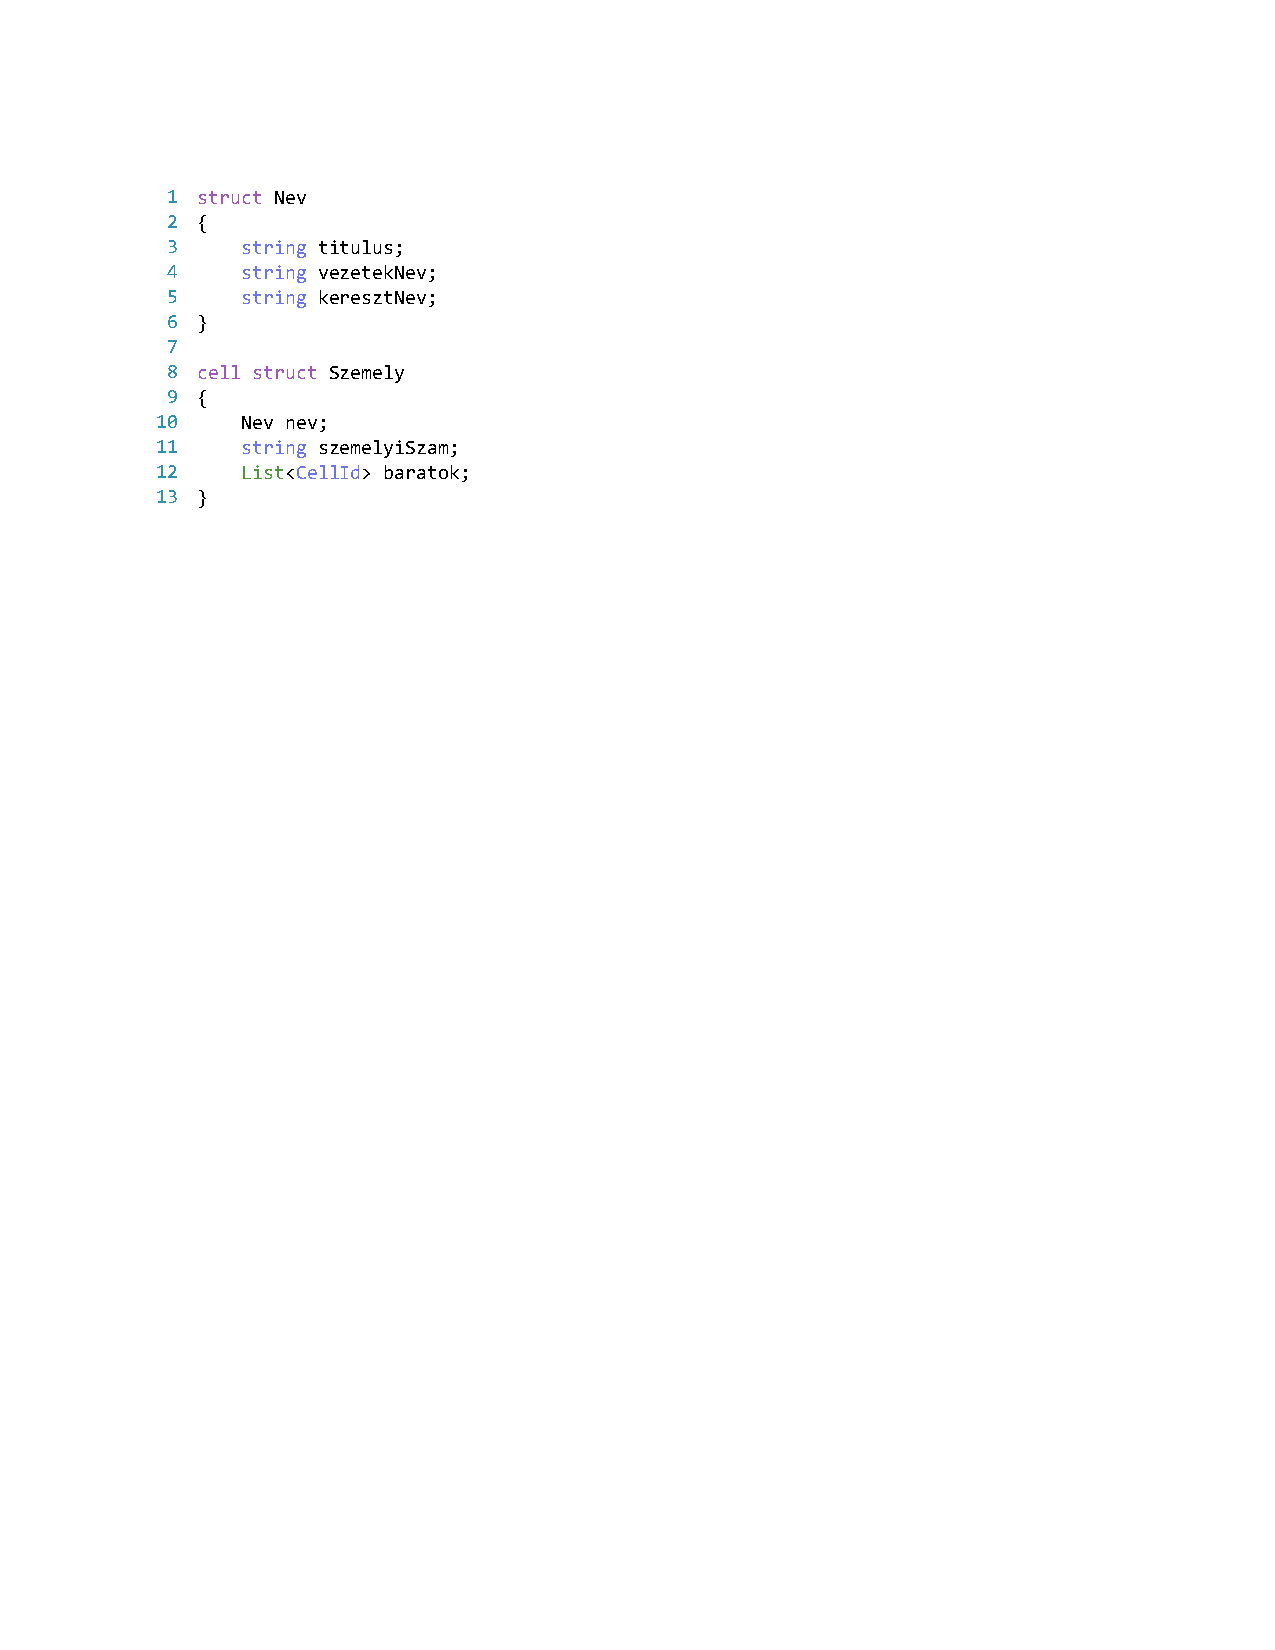
\includegraphics[]{figures/TarsasagTSL.pdf}
	\caption{Példa TSL használatára.}
	\label{fig:TSL}
\end{figure}

\section{Adatelérés}

A Graph Engine a \texttt{cell} típushoz készít úgynevezett \emph{Accessor}-okat, melyek az adatolvasást és manipulálást könnyítik meg. Ezzel párhuzamosan létrehoz osztályokat, amiket a Visual Studioban lévő IntelliSense is tud kezelni, megkönnyítve a további implementációs munkát. Az \emph{Accessor}-ok használatát is a fenti példán keresztül mutatjuk be. Fordítás után a következő metódusokat tudjuk használni: 
\begin{itemize}
	\item \texttt{Global.LocalStorage.IsSzemely(long cellId)} \--- A \emph{cellId} azonosítójú elemről megállapítja, hogy Szemely típusú-e. Visszatérési értéke: \texttt{bool}.
	\item \texttt{Global.LocalStorage.LoadSzemely(long cellId)} \--- Visszatérési értéke egy Szemely típusú objektum, aminek a CellId-je a függvény bemeneteként megadott paraméter.
	\item \texttt{Global.LocalStorage.SaveSzemely(\ldots{})} \--- A függvény bemeneti paraméterének megadott adatok alapján elment egy személyt az adatbázisba. Ez a paraméter lehet Szemely típusú objektum, de megadhatjuk felsorolva az osztály mezőit (\texttt{cellId, nev, szemelyiSzam, baratok}) is. Amennyiben létezik az adott \texttt{cellId}-vel rendelkező bejegyzés, akkor felülírja.
	\item \texttt{Global.LocalStorage.Szemely\_Selector()} \--- Visszatérési értéke egy IEnumerable<Szemely> lista, amiben az adatbázisban szereplő összes személy benne van. Végigiterálva ezen a listán, megkaphatjuk a személyek adatait.
	\item \texttt{Global.LocalStorage.Szemely\_Accessor\_Selector()} \--- Hasonló a \texttt{Szemely\_Selector}-hoz, ellenben IEnumerable<SzemelyAccessor>-ral tér vissza, azaz nem személy osztályú elemekkel, hanem azok \emph{Accessor}-aival.
	\item \texttt{Global.LocalStorage.UseSzemely(long cellId)} \--- Az adott \emph{cellId}-vel rendelkező személy \emph{Accessor}-át adja vissza. Ezen keresztül tudjuk módosítani a bejegyzést. Használat után mindenképp fel kell szabadítani, ezért \emph{using} blokkba érdemes illeszteni.
\end{itemize}

Sajnálatos módon a Graph Engine egyelőre nem támogatja az egymásba ágyazott \emph{Accessor}-ok használatát. Emiatt amennyiben két ember adatait szeretnénk összehasonlítani, akkor először az egyik, majd a másik adatait kell kimentenünk a lokális memóriába, majd összehasonlítani. Erre a problémára megoldást nyújthat a \emph{Language-Integrated Query (LINQ)}, illetve \emph{Language Integrated Knowledge Query (LIKQ)} használata, melyek lehetőséget kínálnak lekérdezések írására.

\subsection{LINQ} \label{graphenginelinq}

A \emph{Language-Integrated Query}, azaz \emph{LINQ} a .NET 3.5 óta létező szolgáltatás, ami megkönnyíti az adatelérést a programozó számára. Célja a nem, vagy csak részben objektum-orientált adatforrások általános célú feldolgozása.\cite{LINQ} Kezdetben az \emph{SQL}- és az \emph{XML} nyelvet támogatta, mivel a relációs adatbázisok és az XML fájlok a két legelterjedtebb, nem objektum-orientált adatforrás.

\begin{figure}[H]
	\centering
	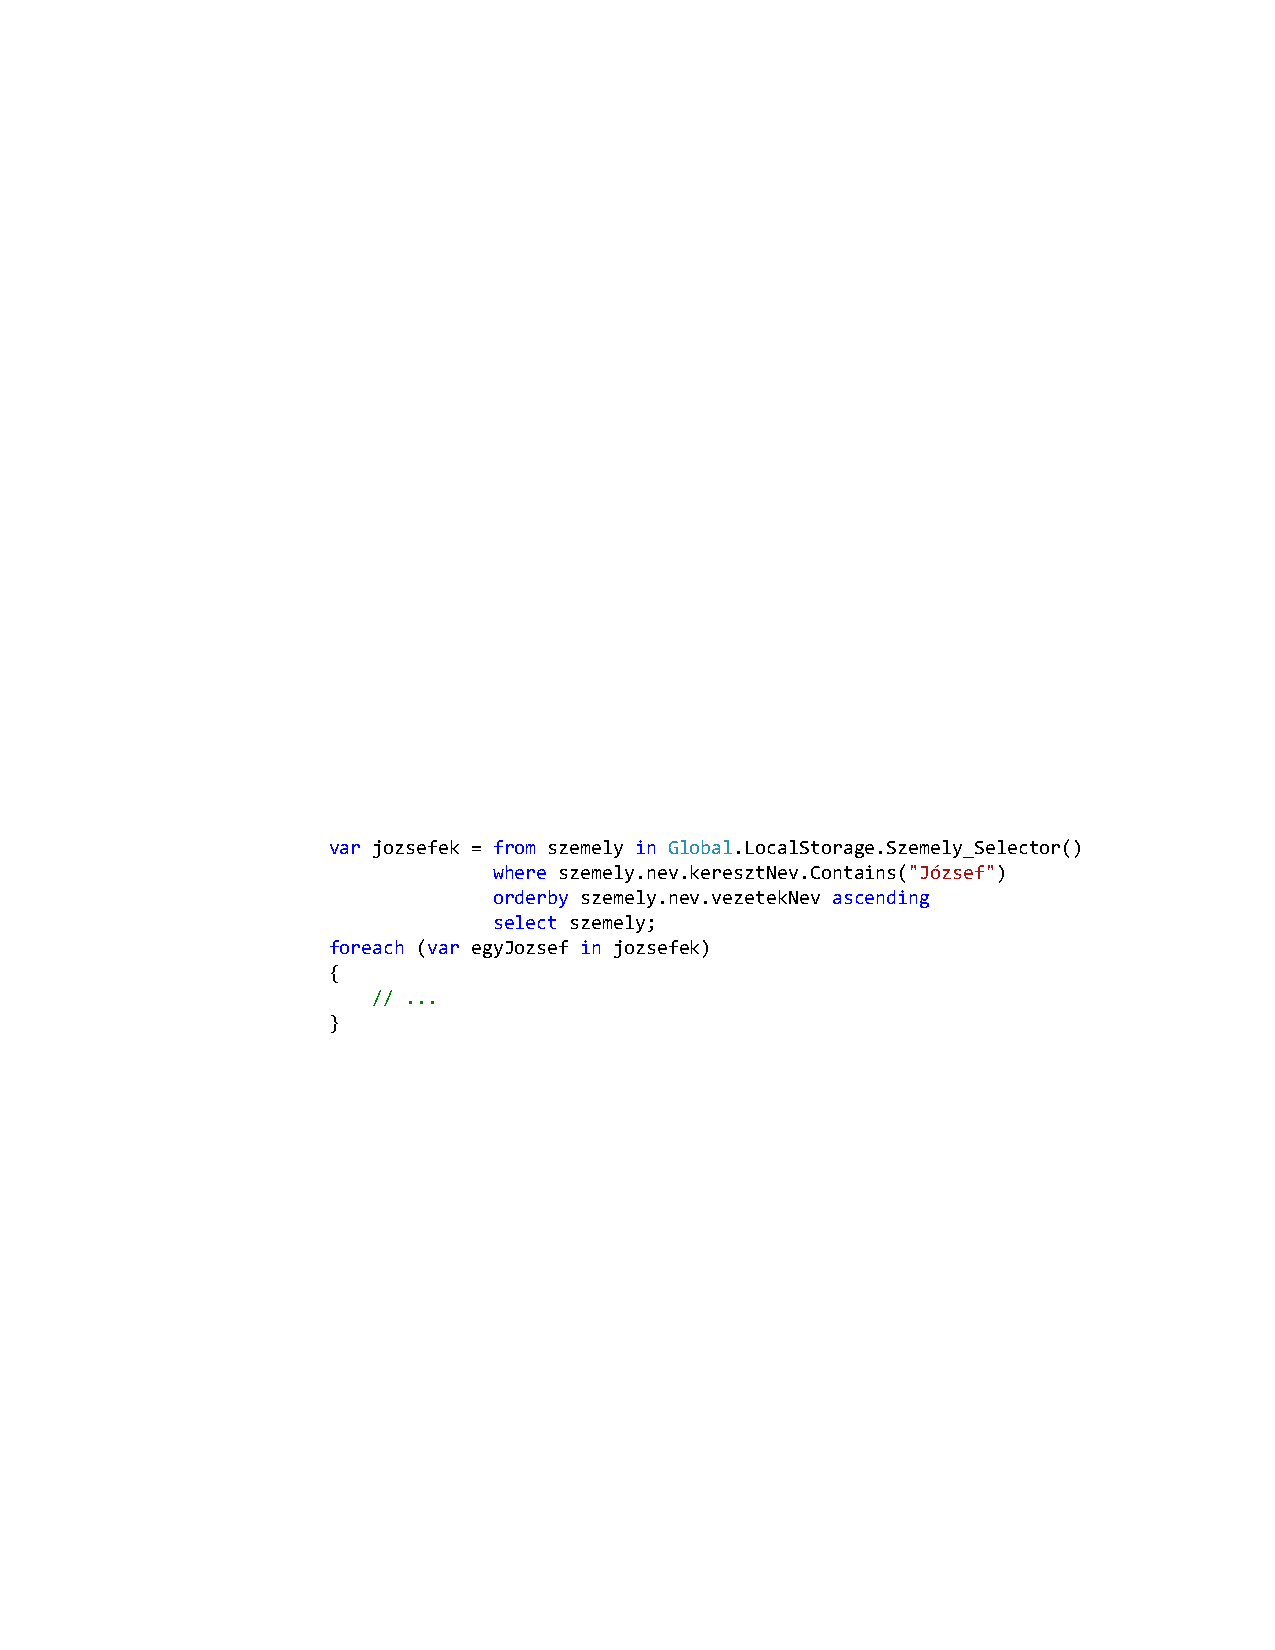
\includegraphics[]{figures/JozsefekLINQ.pdf}
	\caption{Egy egyszerű LINQ lekérdezés. A József keresztnevű emberek adatait lehet kinyerni így.}
	\label{fig:LINQ}
\end{figure}

A \ref{fig:LINQ} ábrán láthatunk egy példát \emph{LINQ} lekérdezésre. Felépítése hasonló az \emph{SQL} nyelv szintaxisához. A \emph{from, where, orderby, select} kulcsszavaknak a jelentése megegyezik. Legfőbb különbség azonban, hogy míg az \emph{SQL}-nél először azt kell megadni, hogy mit szeretnénk, aztán pedig, hogy honnan, addig a \emph{LINQ}-nél ez fordítva van. Ez nagy előny, mivel így az \emph{IntelliSense} már felajánlja az adott osztály mezőit, függvényeit kiegészítésként, emellett fordítás előtt ellenőrizni lehet az esetleges elgépeléseket. A \emph{select} után megadhatunk \emph{property}-ket, anonym-osztályt, de akár, ahogy a \refstruc{fig:LINQ} mutatja, a teljes osztályt is.

A Graph Engine nem támogatja teljes mértékben a lekérdezéseket. Számunkra a legnagyobb hátrány az, hogy nem használható a \emph{join} operátor és nem lehet különböző típusú cellákat egy lekérdezésbe kapcsolni. Ennek oka ugyanaz, amiért nem lehet egymásba ágyazott \emph{Accessor}-okat használni. Ez pedig az, hogy egy \emph{Accessor} elérésnél az adatbázis egészére elhelyez egy zárat. A \emph{LINQ} pedig a \emph{join} műveletnél mindkét \emph{Selector}-nál megpróbál elhelyezni zárat.

A \emph{join} művelet hiánya abban az esetben jelenthet problémát, amikor különböző típusú csúcsok között szeretnénk navigálni. Erre a nehézségre és egy lehetséges megoldására mutatunk egy példát a következő szakaszban.

\subsubsection{Példaalkalmazás}

Egészítsük ki az eddigi példánkat azzal, hogy adatokat tárolunk a személyek háziállatairól is. Tároljuk az állat faját nevét és azt, hogy ki a gazdája. Ehhez a \emph{TSL} fájlt a következőképpen egészítettük ki:

\begin{figure}[H]
	\centering
	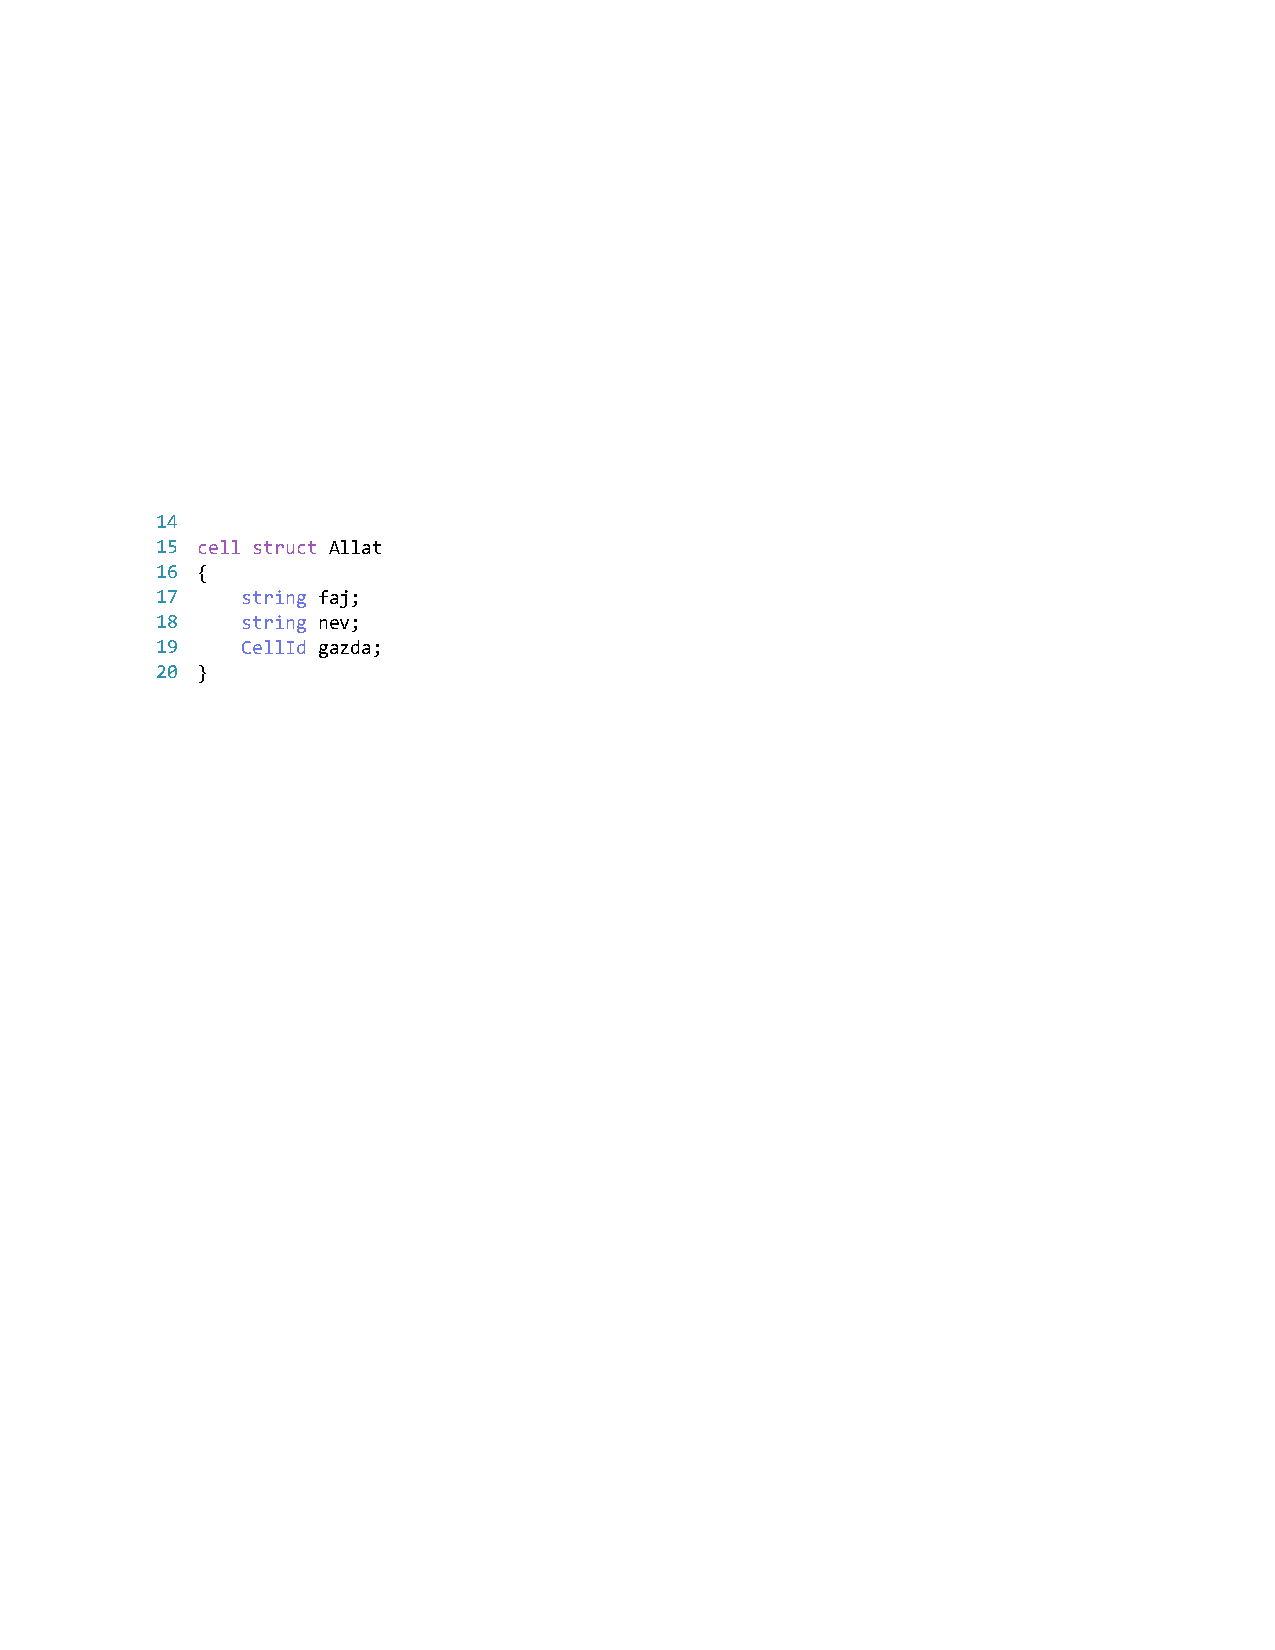
\includegraphics[]{figures/TarsasagAllatTSL.pdf}
	\caption{Kiegészítjük a \emph{TSL} fájlunkat ezekkel a sorokkal, hogy az állatokról is tudjunk adatokat tárolni.}
	\label{fig:TarsasagAllat}
\end{figure}

Egy kézenfekvő kérdés, hogy egy adott nevű személy háziállatait hogy hívják. Ez a látszólag egyszerű kérdés rávilágít arra, hogy miért jelent problémát, hogy nem tudjuk összekapcsolni a különböző típusok \emph{Selector}-át. A nyilvánvaló az lenne, ha egy lekérdezésben meg tudnánk ezt tenni, mint ahogy a \ref{fig:Haziallatok} mutatja, ez viszont kizárólag \emph{LINQ} használatával nem lehetséges.

\begin{figure}[H]
	\centering
	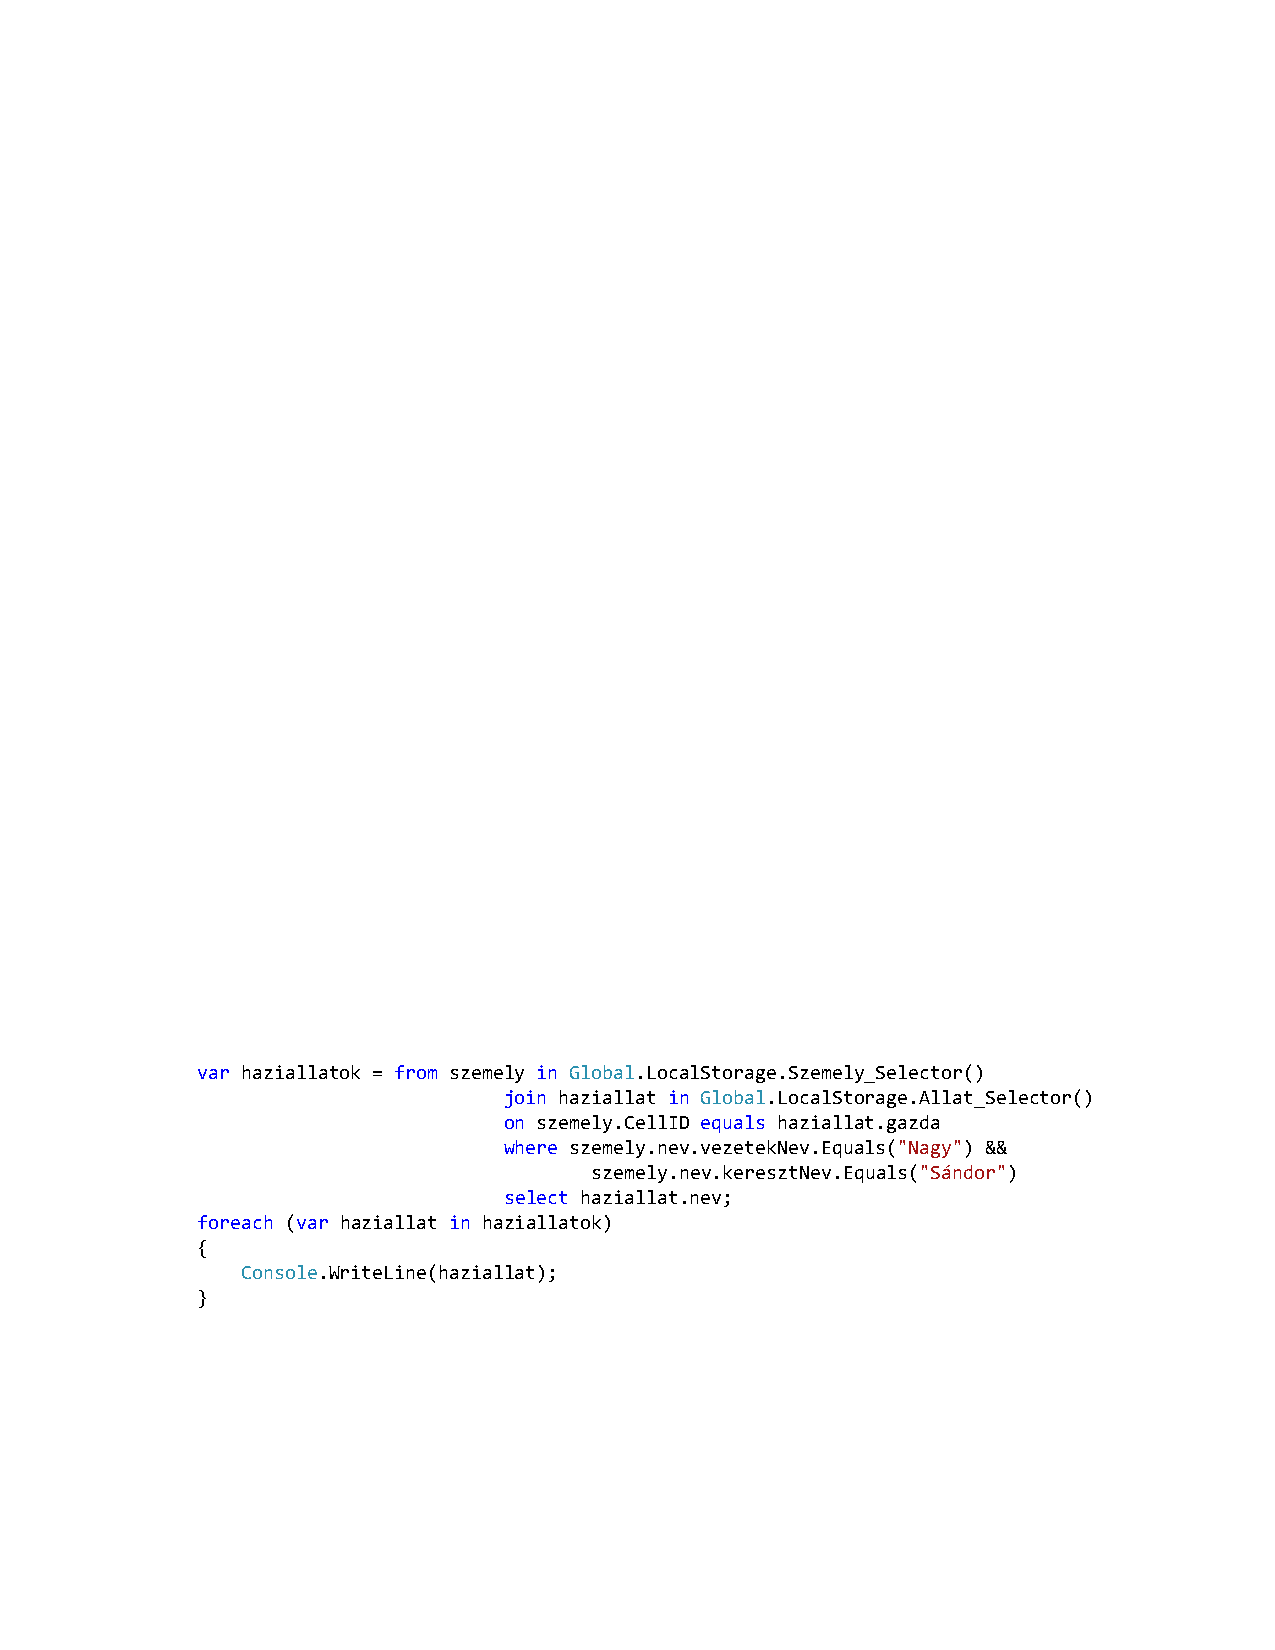
\includegraphics[]{figures/HaziallatokLINQ.pdf}
	\caption{Egy nem támogatott \emph{LINQ} lekérdezés.}
	\label{fig:Haziallatok}
\end{figure}

Az sem jelent megoldást a problémára, hogy lekérdezzük a \emph{Szemely\_Selector}-ral a kívánt személy \emph{CellId}-ját, majd az \emph{Allat\_Selector}-ral a hozzátartozó háziállatok nevét. Mivel a \emph{Selector}-ok zárat helyeznek el az adatbázison, az első lekérdezés után ki kell menteni az adatokat egy másik változóba, különben a második \emph{Selector} nem fogja tudni elérni az adatbázist. Így a megoldás menete a következő:

\begin{itemize}
	\item Első \emph{LINQ} lekérdezés. A \emph{Szemely\_Selector} segítségével megkeressük a "Nagy Sándor" nevű személy \emph{CellId}-jét. Ebben a lépésben a \emph{Selector} hívás miatt zár kerül az adatbázisra.
	\item Létrehozunk egy \emph{long} típusú változót és a kapott \emph{CellId} értékével egyenlővé tesszük.
	\item Feloldódik az adatbáziszár, ezért következhet a második \emph{LINQ} lekérdezés, ahol a háziállatok \emph{Selector}-át használjuk.
	\item Végigiterálunk a háziállatokon és kiírjuk őket.
\end{itemize}

Ez a megkötés rendkívül megnöveli a lekérdezések erőforrásigényét, ugyanis sok esetben az adatokat legalább kétszer kell tárolnunk. A fenti példában csak a személy \emph{CellId}-ját tároltuk lokálisan és az adatbázisban is, de más esetben szükség lehet sok olyan adat lokális tárolására is, amire egyáltalán nincs szükségünk ezáltal fölöslegesen terhelve a memóriát. Emellett a sok lekérdezés a számításigényt is jelentősen növeli.

\subsection{LIKQ}

A \emph{Language-Integrated Knowledge Query} (\emph{LIKQ}) egy projekt, melynek célja egy Graph Engine-hez fejlesztett nyelv, mellyel gráfokat lehet bejárni. Szintaxisa miatt könnyebben érthető lekérdezéseket lehet leírni vele, mint a \emph{LINQ} lekérdezéssel. Egy tudásgráfból épül fel, melyen lehet navigálni. A lekérdezések 3 függvényből épülnek fel, ezek egymás után fűzésével lehet leírni egy lekérdezést. A függvények:

\begin{itemize}
	\item \texttt{StartFrom(long cellId)}
	\item \texttt{FollowEdge(string s)}
	\item \texttt{VisitNode(Expression ex)}
\end{itemize}

Az \emph{Expression ex} egy lambda kifejezést jelent.\cite{Lambda} A dolgozat készítésekor ez a projekt még fejlesztés alatt állt, még nem készült hozzá dokumentáció, ellenben a projekt nyílt forráskódú, így lehetőség van a forráskód tanulmányozására. Ez nem vezetett eredményre, a legegyszerűbb lekérdezésekre sem adott eredményt, \emph{System.NullReferenceException} kivételt dobott minden esetben. Így az implementáció során a munka a \emph{LINQ} lekérdezések használatát követelte meg.